\documentclass[11pt,a4paper]{article}

% ---------------------------------------------------------------------------
% Rapport du projet « Diffusion thermique et géométries fractales »
% Compilation : make rapport (ou latexmk -pdf rapport.tex dans docs/rapport)
% Figures : python3 docs/rapport/figures/generer_figures.py (depuis la racine)
% ---------------------------------------------------------------------------

\usepackage[T1]{fontenc}
\usepackage[utf8]{inputenc}
\usepackage[french]{babel}
\usepackage{lmodern}
\usepackage{microtype}
\usepackage[margin=2.4cm]{geometry}
\usepackage{amsmath,amssymb,amsthm,mathtools}
\usepackage[locale=FR]{siunitx}
\usepackage{booktabs}
\usepackage{graphicx}
\usepackage{float}
\usepackage{caption}
\usepackage{xcolor}
\usepackage{tikz}
\usetikzlibrary{arrows.meta,calc,decorations.pathreplacing}
\usepackage{listings}
\usepackage{enumitem}
\usepackage[french,ruled,vlined,linesnumbered]{algorithm2e}
\usepackage[colorlinks=true,linkcolor=blue!50!black,urlcolor=blue!50!black,citecolor=blue!50!black]{hyperref}
\usepackage[french,noabbrev]{cleveref}

\newtheorem{proposition}{Proposition}
\crefname{proposition}{proposition}{propositions}
\theoremstyle{remark}
\newtheorem*{remarque}{Remarque}

\graphicspath{{figures/}{../captures/}}
\sisetup{per-mode=symbol, inter-unit-product=\ensuremath{\cdot}}


\lstset{
  language=C, basicstyle=\ttfamily\small, keywordstyle=\color{blue!60!black}\bfseries,
  commentstyle=\color{green!40!black}\itshape, stringstyle=\color{red!50!black},
  numbers=left, numberstyle=\tiny\color{gray}, frame=single, framerule=0.3pt,
  breaklines=true, columns=fullflexible, keepspaces=true, xleftmargin=1.5em
}

\newcommand{\dx}{\Delta x}
\newcommand{\dt}{\Delta t}
\newcommand{\Text}{T_{\mathrm{ext}}}
\newcommand{\Tair}{T_{\mathrm{air}}}
\newcommand{\Rsi}{R_{\mathrm{si}}}
\newcommand{\Rse}{R_{\mathrm{se}}}
\newcommand{\la}{\lambda_{\mathrm{air}}}
\newcommand{\lm}{\lambda_{\mathrm{m}}}

\title{\textbf{Diffusion thermique et géométries fractales}\\[0.4em]
\large Une pièce en flocon de Koch évacue-t-elle mieux la chaleur qu'une pièce carrée ?\\
Modèle physique, mathématiques, méthodes numériques et implémentation}
\author{Devrim Genc}
\date{Novembre 2026}

\begin{document}
\maketitle

\begin{abstract}
On compare, à aire égale, une pièce carrée et des pièces dont le contour est un
flocon de Koch de profondeur 0 à 4, chauffées par une même source et entourées de
murs en béton. La grandeur étudiée est la conductance de l'enveloppe
$G = P/(\Tair-\Text)$, la chaleur évacuée par degré d'écart avec l'extérieur. Le
modèle résout l'équation de la chaleur en deux dimensions par volumes finis, dans
l'air (brassé par la convection, représentée par une conductivité effective) et
dans les murs, avec les résistances superficielles normalisées. Il est intégré en
temps par un schéma implicite à directions alternées (Douglas-Rachford, algorithme
de Thomas), et son régime établi est obtenu directement par gradient conjugué.
Deux corrections géométriques éliminent les biais de la grille cartésienne. Le code
est validé sur une solution exacte et par convergence en maillage. Résultat : à
même puissance, le flocon de profondeur 3 reste à \qty{26,0}{\degreeCelsius} contre
\qty{30,0}{\degreeCelsius} pour le carré ($G$ supérieure de \qty{66}{\percent}),
mais le gain s'inverse à la profondeur 4 : l'épaisseur du mur limite physiquement
la fractale.
\end{abstract}

\tableofcontents
\newpage

% ===========================================================================
\section{Introduction}
% ===========================================================================

\subsection{Contexte et problématique}

Dans un monde qui se réchauffe, évacuer la chaleur sans climatisation devient un
enjeu de l'architecture. La géométrie y joue un rôle : à volume égal, une forme dont
la surface est plus grande échange davantage de chaleur avec l'extérieur. Les
fractales poussent cette idée à l'extrême : le flocon de Koch a un périmètre infini
pour une aire finie.

Il faut préciser le sens de cet avantage. Pour une enveloppe d'habitation, plus de
surface signifie plus de pertes en hiver et plus d'apports en canicule : la règle de
l'architecture bioclimatique est la compacité. La fractale n'a donc d'intérêt que
comme \emph{échangeur} : une façade, un mur ou un dissipateur chargé d'évacuer une
chaleur produite à l'intérieur (occupants, équipements, serveurs) vers un milieu plus
froid (air nocturne, sol). D'où la question étudiée :

\begin{center}
\fbox{\parbox{0.86\linewidth}{\centering\itshape
À aire égale, de combien une géométrie fractale augmente-t-elle la chaleur évacuée
passivement, et à quelles conditions ?}}
\end{center}

\subsection{Démarche}

Le projet est né d'un modèle écrit en classe préparatoire, puis repris pour en faire
une base solide. Cette reprise a d'abord consisté à \emph{vérifier} le modèle
existant : chaque hypothèse a été confrontée à la physique, et le code à des
solutions exactes. Plusieurs défauts sont ainsi apparus (\cref{sec-defauts}) : une
confusion entre diffusivité et conductivité, de l'air immobile au lieu d'air brassé,
des murs d'un pixel dont la résistance était fausse de \qty{15}{\percent}, une
précision \texttt{float} qui figeait le calcul, et deux biais de la grille
cartésienne. Le modèle actuel (version~4) corrige ces points et sert de fondation à
la suite du projet, notamment le passage en trois dimensions.

\subsection{Plan}

La \cref{sec-physique} pose le modèle physique, la \cref{sec-koch} étudie le flocon
de Koch. Les \cref{sec-espace,sec-temps} décrivent la discrétisation en espace puis
en temps, avec les algorithmes et leurs propriétés. La \cref{sec-implementation}
présente le code, la \cref{sec-validation} sa validation et la
\cref{sec-resultats} les résultats. La \cref{sec-limites} discute les limites et les
suites.

% ===========================================================================
\section{Modèle physique}\label{sec-physique}
% ===========================================================================

\subsection{Équation de la chaleur}

Dans un milieu de masse volumique $\rho$, de capacité thermique massique $c$ et de
conductivité $\lambda$, la température $T(\mathbf{x},t)$ vérifie
\begin{equation}\label{eq-chaleur}
\rho c\,\frac{\partial T}{\partial t} = \nabla\cdot\big(\lambda\nabla T\big) + s,
\end{equation}
où $s$ est une puissance volumique apportée (\unit{\watt\per\cubic\metre}). Elle
traduit la conservation de l'énergie et la loi de Fourier $\mathbf{q}=-\lambda\nabla T$
pour la densité de flux $\mathbf{q}$ (\unit{\watt\per\square\metre}).

Deux grandeurs ne doivent pas être confondues :
\begin{itemize}
  \item la \emph{conductivité} $\lambda$ (\unit{\watt\per\metre\per\kelvin}) fixe les
  flux, donc tout le régime établi ($\partial_t T = 0$) ;
  \item la \emph{diffusivité} $\alpha = \lambda/(\rho c)$ (\unit{\square\metre\per\second})
  fixe la vitesse des évolutions, et seulement elle.
\end{itemize}
Le modèle de départ utilisait $\alpha$ à la place de $\lambda$, avec $\rho c = 1$
partout. Or les deux rapports n'ont rien à voir : le béton diffuse environ 25 fois
moins vite que l'air immobile ($\alpha$), mais conduit environ 70 fois mieux
($\lambda$). Le modèle de départ représentait donc un mur dix fois moins conducteur
que l'air, l'inverse de la réalité, et ses conclusions en régime établi étaient
faussées.

\subsection{Hypothèses géométriques}

On étudie une coupe horizontale de la pièce : le problème est bidimensionnel, et
toutes les grandeurs sont données \emph{par mètre de hauteur} (puissances en
\unit{\watt\per\metre}, conductances en \unit{\watt\per\metre\per\kelvin}). Le sol et
le plafond sont supposés adiabatiques. La pièce a une aire intérieure de
\qty{36}{\square\metre} quelle que soit sa forme ; elle est entourée d'un mur de
béton de \qty{20}{\centi\metre}, et l'extérieur est un thermostat à
$\Text = \qty{20}{\degreeCelsius}$.

\subsection{L'air brassé}

L'air d'une pièce chauffée n'est pas immobile : la convection le mélange. Résoudre
la mécanique des fluides sortirait du cadre du projet ; on représente le brassage
par une \emph{conductivité effective} $\la$, très supérieure à celle de l'air
immobile. Son ordre de grandeur se déduit du temps de brassage : une perturbation
diffuse sur une distance $R$ en un temps $\tau \sim R^2/\alpha$. Une pièce de
\qty{3}{\metre} de rayon se brasse en quelques minutes ; avec
$\la = \qty{100}{\watt\per\metre\per\kelvin}$ et $\rho c = \qty{1206}{\joule\per\cubic\metre\per\kelvin}$,
\[
\alpha_{\mathrm{air}} = \frac{100}{1206} \approx \qty{0,083}{\square\metre\per\second},
\qquad \tau \approx \frac{3^2}{0,083} \approx \qty{110}{\second} \approx 2~\text{minutes}.
\]
L'air n'est donc pas uniforme : il est plus chaud près de la source (d'environ
\qty{3}{\degreeCelsius} au-dessus de la moyenne en régime établi), et la chaleur
doit le traverser pour atteindre les murs. Ce choix est un paramètre du modèle,
discuté en \cref{sec-limites}.

\begin{remarque}
La version~3 du modèle réduisait l'air à une seule température (un nœud brassé
parfaitement), méthode courante en thermique du bâtiment. Physiquement acceptable,
elle supprimait toute diffusion visible dans la pièce, alors que la simulation sert
aussi à visualiser le phénomène. La version~4 résout donc l'air sur la grille.
\end{remarque}

\subsection{Murs et échanges superficiels}

Contre une paroi, l'air forme une couche limite où les échanges convectifs et
radiatifs se résument par une \emph{résistance superficielle} $R_s$
(\unit{\square\metre\kelvin\per\watt}). La norme ISO~6946 donne, pour un flux
horizontal, $\Rsi = \num{0,13}$ côté intérieur et $\Rse = \num{0,04}$ côté
extérieur. Le flux traversant une surface s'écrit alors
$q = \Delta T / R_s$, ce qui donne une condition de Robin aux interfaces.

Pour un mur plan d'épaisseur $e$, les trois résistances sont en série ; le
coefficient de transmission vaut
\begin{equation}\label{eq-U}
U = \frac{1}{\Rsi + e/\lm + \Rse}
  = \frac{1}{0,13 + 0,20/1,75 + 0,04}
  \approx \qty{3,52}{\watt\per\square\metre\per\kelvin}.
\end{equation}
Un mètre de mur droit (sur un mètre de hauteur) transmet donc environ
\qty{3,5}{\watt} par kelvin d'écart entre l'air contre la paroi et l'extérieur.

\subsection{Source de chaleur et grandeur étudiée}

Une source (radiateur, appareil) occupe un disque de \qty{30}{\centi\metre} de rayon
centré sur le centre de gravité de la pièce et injecte
$Q = \qty{800}{\watt\per\metre}$, soit \qty{2}{\kilo\watt} pour \qty{2,5}{\metre} de
hauteur (environ \qty{55}{\watt\per\square\metre} de plancher).

En intégrant \eqref{eq-chaleur} sur tout le domaine intérieur (air et murs), le
théorème de flux-divergence donne le bilan d'énergie
\begin{equation}\label{eq-bilan}
\frac{\mathrm{d}E}{\mathrm{d}t} = Q - P_{\mathrm{ext}},
\qquad E = \int \rho c\,T\,\mathrm{d}A,
\end{equation}
où $P_{\mathrm{ext}}$ est la puissance sortant par la surface extérieure des murs.
En régime établi, $P_{\mathrm{ext}} = Q$ : toute la chaleur produite ressort. La
comparaison des formes porte sur la \emph{conductance de l'enveloppe}
\begin{equation}\label{eq-G}
G = \frac{P_{\mathrm{ext}}}{\Tair - \Text}\quad(\unit{\watt\per\metre\per\kelvin}),
\end{equation}
où $\Tair$ est la température moyenne de l'air. Plus $G$ est grande, plus la pièce
évacue de chaleur pour un même écart de température ; à puissance donnée, plus elle
reste fraîche.

\subsection{Temps caractéristiques}

Trois échelles de temps coexistent :
\begin{itemize}
  \item le brassage de l'air, environ \qty{2}{\minute} ;
  \item la diffusion à travers le mur : $e^2/\alpha_{\mathrm{m}}$ avec
  $\alpha_{\mathrm{m}} = 1,75/2,3\cdot 10^{6} \approx \qty{7,6e-7}{\square\metre\per\second}$,
  soit environ \qty{15}{\hour} ;
  \item la mise en température globale, de l'ordre de $C_{\mathrm{murs}}/G$. Pour le
  carré, les murs (environ \qty{5}{\square\metre} de section) ont une capacité de
  $\qty{1,1e7}{\joule\per\metre\per\kelvin}$ ; avec $G \approx 80$, on trouve
  $\tau \approx \qty{1,4e5}{\second} \approx \qty{1,6}{jours}$, et le régime établi
  est atteint après quelques $\tau$, soit environ cinq jours, comme observé.
\end{itemize}
La capacité de l'air ($1206 \times 36 \approx \qty{4e4}{\joule\per\metre\per\kelvin}$)
est négligeable devant celle des murs : l'air suit les murs presque instantanément.
Ce rapport d'échelles (minutes contre jours) est au cœur des difficultés numériques
de la \cref{sec-temps}.

% ===========================================================================
\section{Le flocon de Koch}\label{sec-koch}
% ===========================================================================

\subsection{Construction récursive}

On part d'un triangle équilatéral. À chaque profondeur, chaque segment $[A,B]$ est
remplacé par quatre segments : on note $P_3 = A + \tfrac13\overrightarrow{AB}$ et
$P_4 = A + \tfrac23\overrightarrow{AB}$, et le sommet du pic est l'image de $P_4$
par la rotation de centre $P_3$ et d'angle $-\pi/3$ :
\[
\text{pic} = P_3 + R_{-\pi/3}\Big(\tfrac13\overrightarrow{AB}\Big),\qquad
R_\theta = \begin{pmatrix}\cos\theta & -\sin\theta\\ \sin\theta & \cos\theta\end{pmatrix}.
\]
Le segment devient $[A,P_3]$, $[P_3,\text{pic}]$, $[\text{pic},P_4]$, $[P_4,B]$, et
la construction se poursuit récursivement sur chacun. Le code
(\texttt{koch\_side} dans \texttt{geometry.c}) calcule tous les sommets en
flottants et produit un polygone exact de $3\cdot 4^n$ sommets.

\subsection{Périmètre et aire}

\begin{proposition}\label{prop-koch}
Soit $s$ le côté du triangle initial et $A_0 = \frac{\sqrt3}{4}s^2$ son aire. Le
flocon de profondeur $n$ a pour périmètre et pour aire
\[
P_n = 3s\left(\frac43\right)^{n},\qquad
A_n = A_0\left(\frac85 - \frac35\left(\frac49\right)^{n}\right).
\]
\end{proposition}

\begin{proof}
À la profondeur $n$, le contour compte $N_n = 3\cdot4^n$ segments de longueur
$\ell_n = s/3^n$, d'où $P_n = N_n\ell_n = 3s(4/3)^n$. Passer de la profondeur $k-1$
à $k$ ajoute un triangle équilatéral de côté $\ell_k = s/3^k$ sur chacun des
$N_{k-1} = 3\cdot4^{k-1}$ segments, soit une aire
$3\cdot4^{k-1}\cdot A_0/9^k = \frac34 A_0 \left(\frac49\right)^k$. En sommant la
série géométrique,
\[
A_n = A_0\left(1 + \frac34\sum_{k=1}^{n}\left(\frac49\right)^k\right)
    = A_0\left(1 + \frac34\cdot\frac49\cdot\frac{1-(4/9)^n}{1-4/9}\right)
    = A_0\left(1 + \frac35\Big(1-\big(\tfrac49\big)^n\Big)\right). \qedhere
\]
\end{proof}

Quand $n\to\infty$, le périmètre tend vers l'infini alors que l'aire tend vers
$\frac85A_0$. La courbe limite a pour dimension de similarité
$\ln 4/\ln 3 \approx 1,26$ : chaque morceau est fait de 4 copies réduites d'un
facteur 3.

\subsection{Pièces de même aire}

Pour comparer les formes à aire égale $A = \qty{36}{\square\metre}$, on règle le
rayon $r$ du cercle circonscrit au triangle initial. Comme $s = r\sqrt3$ et
$A_0 = \frac{3\sqrt3}{4}r^2$, la \cref{prop-koch} donne
\[
r_n = \sqrt{\frac{A}{f(n)\,\frac{3\sqrt3}{4}}},\qquad f(n) = \frac85-\frac35\Big(\frac49\Big)^n.
\]
Le carré a pour côté $\sqrt{A} = \qty{6}{\metre}$. La \cref{fig-koch} montre les six
formes ; le périmètre passe de \qty{24}{\metre} (carré) à \qty{68,9}{\metre}
(profondeur 4).

\begin{figure}[H]
\centering
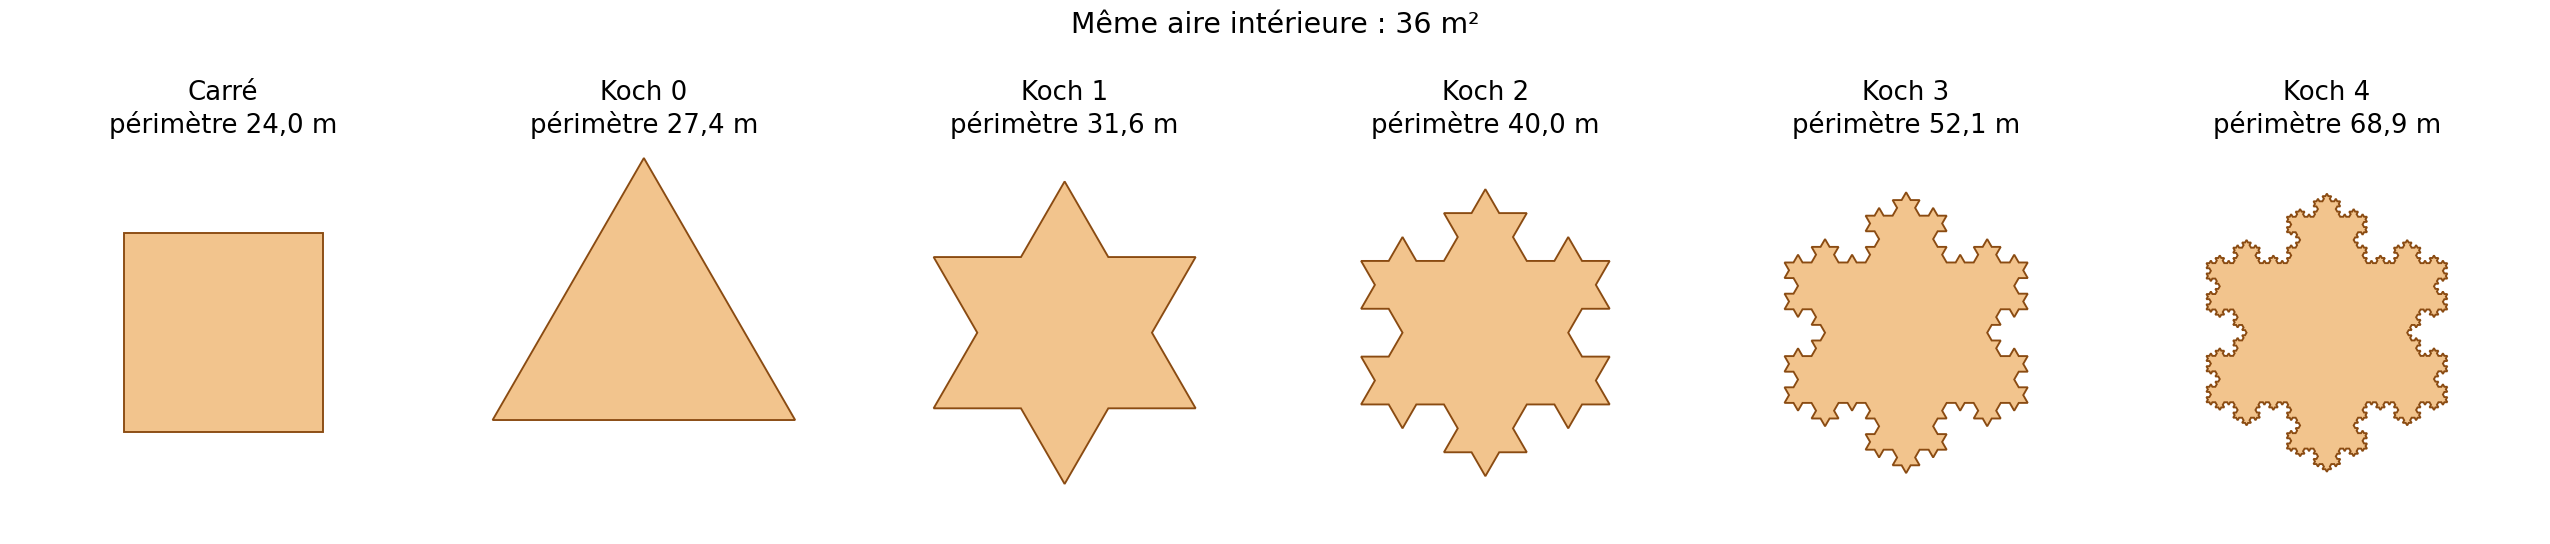
\includegraphics[width=\linewidth]{koch_profondeurs.png}
\caption{Carré et flocons de Koch de profondeur 0 à 4, tous d'aire intérieure
\qty{36}{\square\metre}.}
\label{fig-koch}
\end{figure}

\subsection{Taille des détails et épaisseur du mur}\label{sec-nmax}

Le segment élémentaire mesure $\ell_n = s_n/3^n$. Pour des pièces de
\qty{36}{\square\metre} :

\begin{center}
\begin{tabular}{lccccc}
\toprule
Profondeur $n$ & 0 & 1 & 2 & 3 & 4\\
\midrule
Côté du triangle $s_n$ (m) & 9,12 & 7,84 & 7,49 & 7,33 & 7,26\\
Segment $\ell_n$ & \qty{9,1}{\metre} & \qty{2,6}{\metre} & \qty{83}{\centi\metre} & \qty{27}{\centi\metre} & \qty{9}{\centi\metre}\\
\bottomrule
\end{tabular}
\end{center}

Un mur fait \qty{20}{\centi\metre}. À la profondeur 3, les détails ont déjà la taille
du mur ; à la profondeur 4, ils sont plus fins que lui. La profondeur au-delà de
laquelle les détails deviennent plus petits que le mur vérifie
$s/3^n \approx e$, soit $n_{\max} \approx \log_3(s/e) \approx \log_3(7,3/0,2)
\approx 3,3$. Pour une pièce, la plage physiquement pertinente est donc
$0\le n\le 3$ ; c'est l'origine de l'optimum observé en \cref{sec-resultats}.

% ===========================================================================
\section{Discrétisation en espace}\label{sec-espace}
% ===========================================================================

\subsection{Grille et zones}

Le domaine est une grille carrée de $N_g\times N_g$ cases de côté $\dx$ : $300\times300$
cases de \qty{3,5}{\centi\metre} pour la fenêtre (domaine de \qty{10,5}{\metre}),
$1200\times1200$ cases de \qty{1,25}{\centi\metre} pour les résultats précis.
Chaque case reçoit une zone à partir du polygone exact du contour intérieur :
\begin{itemize}
  \item \textbf{air} si son centre est dans le polygone (test pair-impair : on compte
  les côtés traversés par une demi-droite horizontale issue du point) ;
  \item \textbf{mur} si elle est hors du polygone et à une distance du contour
  inférieure à $e = \qty{20}{\centi\metre}$ (distance minimale aux segments,
  par projection orthogonale bornée) ;
  \item \textbf{extérieur} sinon.
\end{itemize}
Le mur est ainsi la \emph{dilatation} du contour vers l'extérieur : il comble les
creux plus étroits que son épaisseur, ce qui reproduit la limite physique de la
\cref{sec-nmax}. Les deux tests coûtent $O(n_{\mathrm{poly}})$ par case ; on ne les
applique qu'aux cases du rectangle englobant élargi de $e$. La source est le disque
de rayon \qty{30}{\centi\metre} centré sur le centre de gravité du polygone, calculé
par les formules
\[
\mathcal{A} = \frac12\sum_k (x_k y_{k+1} - x_{k+1}y_k),\qquad
x_G = \frac{1}{6\mathcal{A}}\sum_k (x_k + x_{k+1})(x_k y_{k+1} - x_{k+1}y_k),
\]
et de même pour $y_G$. La puissance $Q$ est répartie également entre ses cases.

\subsection{Volumes finis}

On intègre \eqref{eq-chaleur} sur une case $i$ (par mètre de hauteur). Avec la
température moyenne $T_i$ et le théorème de flux-divergence,
\begin{equation}\label{eq-vf}
C_i\,\frac{\mathrm{d}T_i}{\mathrm{d}t} = \sum_{j\in\mathcal{V}(i)} G_{ij}\,(T_j - T_i) + S_i,
\qquad C_i = \rho c\,\dx^2,
\end{equation}
où la somme porte sur les quatre voisins, $S_i$ est la puissance injectée dans la
case, et $G_{ij}$ (\unit{\watt\per\metre\per\kelvin}) est la \emph{conductance de la
face} commune. Une face de longueur $\dx$ entre deux centres distants de $\dx$ est
traversée par des résistances en série (par unité de longueur de face) : une
demi-case de chaque côté, $\dx/(2\lambda)$, et éventuellement une résistance
superficielle. D'où
\begin{equation}\label{eq-conductances}
\begin{aligned}
\text{air/air, mur/mur :}\quad & G = \frac{\dx}{\frac{\dx}{2\lambda_i}+\frac{\dx}{2\lambda_j}},\\
\text{air/mur :}\quad & G = \frac{\dx}{\frac{\dx}{2\la}+\Rsi+\frac{\dx}{2\lm}},\\
\text{mur/extérieur :}\quad & G = \frac{\dx}{\frac{\dx}{2\lm}+\Rse}.
\end{aligned}
\end{equation}
Pour deux cases identiques, $G=\lambda$ ; à l'interface de deux matériaux, on
obtient la moyenne harmonique des conductivités, qui est la bonne moyenne pour des
résistances en série.

\begin{proposition}[conservation]
Le schéma \eqref{eq-vf} conserve l'énergie : $\frac{\mathrm{d}}{\mathrm{d}t}\sum_i C_iT_i
= \sum_i S_i - P_{\mathrm{ext}}$, où $P_{\mathrm{ext}}$ est la somme des flux à
travers les faces mur/extérieur.
\end{proposition}

\begin{proof}
En sommant \eqref{eq-vf}, chaque face intérieure apparaît deux fois, avec
$G_{ij}(T_j-T_i)$ pour $i$ et $G_{ji}(T_i-T_j)$ pour $j$. Comme $G_{ij}=G_{ji}$,
ces termes s'annulent. Il ne reste que les sources et les faces vers l'extérieur.
\end{proof}

C'est la version discrète exacte de \eqref{eq-bilan}. Le code vérifie ce bilan à
chaque simulation : en régime établi, $P_{\mathrm{ext}} = Q$ à la précision machine.

\subsection{Corrections de surface}\label{sec-corrections}

La grille cartésienne introduit deux biais aux surfaces, que les tests de la
\cref{sec-validation} ont mis en évidence.

\paragraph{Facteur d'escalier.} Une surface inclinée d'un angle $\theta$ sur la
grille est une suite de marches (\cref{fig-escalier}). Pour une longueur $L$ de mur,
elle compte $L(|\cos\theta|+|\sin\theta|)/\dx$ faces au lieu de $L/\dx$. Une
résistance superficielle posée sur chaque face surestime donc l'échange d'un
facteur $f = |\cos\theta|+|\sin\theta|$, jusqu'à $\sqrt2$ à \ang{45}. Ce biais ne
dépend pas de $\dx$ : il ne disparaît pas en raffinant la grille.

\begin{figure}[H]
\centering
\begin{tikzpicture}[scale=0.55]
  \foreach \x in {0,...,8} \draw[gray!30] (\x,0) -- (\x,6);
  \foreach \y in {0,...,6} \draw[gray!30] (0,\y) -- (8,\y);
  \fill[blue!12] (0,0) -- (0,6) -- (1,6) -- (1,5) -- (2,5) -- (2,4) -- (3,4) -- (3,3)
    -- (5,3) -- (5,2) -- (6,2) -- (6,1) -- (7,1) -- (7,0) -- cycle;
  \draw[very thick,red!70!black] (1,6) -- (1,5) -- (2,5) -- (2,4) -- (3,4) -- (3,3)
    -- (5,3) -- (5,2) -- (6,2) -- (6,1) -- (7,1) -- (7,0);
  \draw[very thick,blue!70!black,dashed] (0.5,6.25) -- (7.5,-0.25);
  \draw[blue!70!black,-{Stealth}] (8.3,4.6) -- (4.2,2.6);
  \node[blue!70!black,right] at (8.3,4.6) {vraie surface, longueur $L$};
  \draw[red!70!black,-{Stealth}] (8.3,1.6) -- (6.1,1.05);
  \node[red!70!black,right] at (8.3,1.6) {faces de la grille};
  \node at (1.2,1.5) {air};
  \node at (6.8,4.5) {mur};
\end{tikzpicture}
\caption{Une surface inclinée devient un escalier : la longueur des faces vaut
$L(|\cos\theta|+|\sin\theta|)$.}
\label{fig-escalier}
\end{figure}

\begin{proposition}
Pour une surface dont toutes les orientations sont équiprobables (un cercle), le
rapport moyen entre vraie longueur et longueur des faces vaut
\[
\frac{2}{\pi}\int_0^{\pi/2}\frac{\mathrm{d}\theta}{\cos\theta+\sin\theta}
= \frac{2\sqrt2}{\pi}\ln\big(1+\sqrt2\big) \approx 0,794.
\]
\end{proposition}

\begin{proof}
Comme $\cos\theta+\sin\theta = \sqrt2\sin(\theta+\pi/4)$, le changement de variable
$u=\theta+\pi/4$ et une primitive de $1/\sin u$, $\ln\tan(u/2)$, donnent
\[
\int_0^{\pi/2}\frac{\mathrm{d}\theta}{\cos\theta+\sin\theta}
= \frac{1}{\sqrt2}\Big[\ln\tan\frac u2\Big]_{\pi/4}^{3\pi/4}
= \frac{1}{\sqrt2}\ln\frac{\tan(3\pi/8)}{\tan(\pi/8)}
= \sqrt2\,\ln\big(1+\sqrt2\big),
\]
car $\tan(3\pi/8) = 1+\sqrt2$ et $\tan(\pi/8) = \sqrt2-1 = 1/(1+\sqrt2)$.
\end{proof}

Le test de la pièce circulaire retrouve exactement ce facteur (\cref{sec-validation}).
Pour un flocon, dont les murs sont à \ang{0}, \ang{60} et \ang{120}, le biais
favorise la fractale face au carré, dont les murs sont alignés sur la grille.

La correction multiplie la résistance de surface de chaque face par $f$, calculé
avec la vraie normale $\mathbf{n}$ au contour au milieu de la face :
$f = |n_x|+|n_y|$. Pour la surface intérieure, $\mathbf{n}$ est la normale du
segment le plus proche ; pour la surface extérieure (courbe parallèle au contour à
la distance $e$), c'est la direction qui va du point le plus proche du contour au
milieu de la face. La conductance totale d'un escalier est alors celle de sa vraie
longueur.

\paragraph{Correction d'épaisseur.} Les cases sont entières : un mur de
\qty{20}{\centi\metre} sur des cases de \qty{3,5}{\centi\metre} occupe 5 ou 6 cases
selon sa position, et ne mesure par exemple que \qty{17,5}{\centi\metre}. Sur le
carré, cela augmentait $G$ de \qty{5}{\percent}. On calcule pour chaque face de
surface l'épaisseur manquante $\delta$ entre la face et la vraie surface (négative
si la grille met trop de mur), et on ajoute la résistance $\delta/\lm$.

\paragraph{Formule finale.} Pour une face air/mur,
\begin{equation}\label{eq-Gcorr}
G = \frac{\dx}{\dfrac{\dx}{2\la} + \Big(\Rsi + \dfrac{\delta}{\lm}\Big) f + \dfrac{\dx}{2\lm}},
\end{equation}
et de même pour une face mur/extérieur avec $\Rse$ et sans demi-case d'air. Un
garde-fou empêche un excès de mur d'annuler la demi-case de béton.

% ===========================================================================
\section{Discrétisation en temps et solveurs}\label{sec-temps}
% ===========================================================================

Le système \eqref{eq-vf} s'écrit sous forme matricielle
\begin{equation}\label{eq-matriciel}
C\,\frac{\mathrm{d}T}{\mathrm{d}t} = (A_x + A_y)\,T + S,
\end{equation}
où $C$ est la matrice diagonale des capacités, et $A_x$, $A_y$ regroupent les échanges
par les faces verticales et horizontales. Les cases extérieures sont fixées à
$\Text$.

\subsection{Le schéma explicite et sa limite}

Le schéma d'Euler explicite $C(T^{n+1}-T^n)/\dt = (A_x+A_y)T^n + S$ est stable si
et seulement si, pour chaque case, $\dt\sum_j G_{ij} \le C_i$ (condition qui
garantit aussi le principe du maximum). Dans l'air,
$\sum_j G_{ij} = 4\la$ et $C_i = \rho c\,\dx^2$, d'où
\[
\dt \le \frac{\rho c\,\dx^2}{4\la} = \frac{1206\times0,035^2}{400}\approx\qty{0,0037}{\second}.
\]
Atteindre le régime établi (une semaine simulée) demanderait plus de $10^8$ pas :
c'est le problème des systèmes \emph{raides}, où cohabitent des échelles de temps
très différentes (\cref{sec-physique}). Il faut un schéma implicite.

\subsection{Le schéma de Douglas-Rachford}

Un schéma totalement implicite demanderait de résoudre à chaque pas un système de
$N = N_g^2$ inconnues. Les méthodes à directions alternées découpent ce système en
problèmes unidimensionnels. Le schéma de Douglas-Rachford, avec $M = C/\dt$, s'écrit
\begin{equation}\label{eq-dr}
\left\{
\begin{aligned}
(M - A_x)\,T^{\star}  &= (M + A_y)\,T^{n} + S &&\text{(lignes, implicite en $x$)}\\
(M - A_y)\,T^{n+1}    &= M\,T^{\star} - A_y\,T^{n} &&\text{(colonnes, implicite en $y$)}
\end{aligned}
\right.
\end{equation}
$A_x$ ne couple que des cases d'une même ligne : la première étape est un système
tridiagonal par ligne. De même, la seconde est un système tridiagonal par colonne.

\begin{proposition}[régime établi exact]
Si $T^{n+1} = T^n = T$, alors $(A_x+A_y)T + S = 0$ : le régime établi du schéma est
exactement celui de l'équation discrète \eqref{eq-matriciel}, quel que soit $\dt$.
\end{proposition}

\begin{proof}
La seconde équation donne $(M-A_y)T = MT^\star - A_yT$, donc $MT = MT^\star$ et
$T^\star = T$ ($M$ est inversible). La première devient
$(M-A_x)T = (M+A_y)T + S$, soit $-A_xT = A_yT + S$.
\end{proof}

\begin{proposition}[stabilité et amortissement]
Supposons que $M^{-1}A_x$ et $M^{-1}A_y$ commutent, de valeurs propres $-a$ et $-b$
($a,b\ge0$) sur un vecteur propre commun. Le facteur d'amplification d'un pas est
\[
g = \frac{1 + ab}{(1+a)(1+b)} \in\ ]0,1].
\]
\end{proposition}

\begin{proof}
Sur le vecteur propre, en divisant par $M$ : $(1+a)T^\star = (1-b)T^n$, puis
$(1+b)T^{n+1} = T^\star + bT^n = \frac{(1-b) + b(1+a)}{1+a}T^n = \frac{1+ab}{1+a}T^n$.
Enfin $(1+a)(1+b) = 1+ab+a+b \ge 1+ab > 0$.
\end{proof}

Le schéma est donc stable pour tout $\dt$. Mais si $a$ et $b$ sont tous deux grands
devant 1, $g\to1$ : les modes raides ne sont presque plus amortis. C'est le cas dans
l'air, dont la capacité est minuscule devant sa conductance. Avec de grands pas,
les variations rapides de l'air persistent et faussent le champ. On l'a mesuré sur le
carré après six jours simulés :

\begin{center}
\begin{tabular}{lccccccc}
\toprule
$\dt$ (s) & 2 & 10 & 30 & 60 & 120 & 300 & 900\\
\midrule
$T_{\max}$ de l'air (°C) & 33,1341 & 33,1341 & 33,1341 & 33,1341 & 33,1339 & 33,1383 & 33,0134\\
Rugosité (°C) & $10^{-12}$ & $4\cdot10^{-12}$ & $4\cdot10^{-5}$ & $3\cdot10^{-3}$ & $9\cdot10^{-3}$ & $2\cdot10^{-2}$ & $2\cdot10^{-2}$\\
\bottomrule
\end{tabular}
\end{center}

La rugosité est le plus grand laplacien discret dans l'air (hors source). Jusqu'à
\qty{30}{\second}, le champ est exact et lisse ; au-delà, des oscillations
apparaissent. Le pas est donc plafonné à \qty{30}{\second}, et la fenêtre enchaîne
plusieurs pas par image quand elle va vite.

\subsection{L'algorithme de Thomas}

Chaque ligne ou colonne demande de résoudre un système tridiagonal
$a_kx_{k-1}+b_kx_k+c_kx_{k+1} = d_k$, $0\le k<n$ (avec $a_0 = c_{n-1} = 0$). Les
cases extérieures sont des lignes triviales $x_k = \Text$. L'algorithme de Thomas
est l'élimination de Gauss adaptée à cette structure.

\begin{algorithm}[H]
\caption{Algorithme de Thomas}
\Entree{$a,b,c,d$ de taille $n$}
\Sortie{la solution $x$, écrite dans $d$}
$c_0 \leftarrow c_0/b_0$ ;\quad $d_0 \leftarrow d_0/b_0$\;
\Pour(\tcp*[f]{élimination}){$k$ de $1$ à $n-1$}{
  $m \leftarrow b_k - a_k c_{k-1}$\;
  $c_k \leftarrow c_k/m$ ;\quad $d_k \leftarrow (d_k - a_k d_{k-1})/m$\;
}
\Pour(\tcp*[f]{remontée}){$k$ de $n-2$ à $0$}{
  $d_k \leftarrow d_k - c_k d_{k+1}$\;
}
\end{algorithm}

\begin{proposition}
L'algorithme coûte $O(n)$ opérations. Si la matrice est à diagonale strictement
dominante ($|b_k| > |a_k|+|c_k|$), les pivots $m$ ne s'annulent pas et
$|c_k|\le 1$ après normalisation : l'algorithme est bien défini et stable.
\end{proposition}

\begin{proof}
Deux boucles de $n$ itérations à coût constant donnent $O(n)$. Pour la stabilité,
par récurrence : si $|c_{k-1}|\le1$ après normalisation, alors
$|m| \ge |b_k| - |a_k| > |c_k| \ge 0$, donc $m\ne0$ et $|c_k/m| < 1$.
\end{proof}

Dans \eqref{eq-dr}, la diagonale vaut $M_i + G_{i,\mathrm{gauche}} + G_{i,\mathrm{droite}}$
et les termes hors diagonale $-G$ : la dominance est stricte grâce à $M_i>0$. Un pas
de temps coûte donc $O(N)$ : deux passes de $N_g$ systèmes de taille $N_g$. En
pratique, \qty{1}{\milli\second} pour la grille de la fenêtre ($N = 90\,000$).

\begin{lstlisting}[caption={Première étape d'un pas (lignes), extrait de \texttt{physics.c}}]
for (int y = 0; y < G; y++) {
    for (int x = 0; x < G; x++) {
        int i = y * G + x;
        if (s->zones[i] == ZONE_EXT) {          /* thermostat : T = T_EXT */
            a[x] = c[x] = 0.0; b[x] = 1.0; d[x] = s->T[i];
            continue;
        }
        double M = s->cap[i] / dt, kl = s->kx[i - 1], kr = s->kx[i];
        a[x] = -kl;  c[x] = -kr;  b[x] = M + kl + kr;
        d[x] = M * s->T[i] + flux_y(s, i) + s->src[i];   /* (M + A_y) T(n) + S */
    }
    thomas(G, a, b, c, d);
    for (int x = 0; x < G; x++) s->Tstar[y * G + x] = d[x];
}
\end{lstlisting}

\subsection{Le régime établi par gradient conjugué}

Pour les résultats, seul le régime établi compte. Plutôt que de simuler cinq à douze
jours, on résout directement $(A_x+A_y)T + S = 0$. En posant $v = T - \Text$
(nulle sur les cases extérieures), le système devient $Kv = S$ avec
\[
(Kv)_i = \sum_{j\in\mathcal{V}(i)} G_{ij}\,(v_i - v_j),\qquad v_j = 0 \text{ si $j$ est extérieure.}
\]

\begin{proposition}
$K$ est symétrique définie positive.
\end{proposition}

\begin{proof}
La symétrie vient de $G_{ij}=G_{ji}$. Pour tout $v$, en regroupant les termes par face,
\[
v^{\top}Kv = \sum_{\text{faces intérieures}} G_{ij}(v_i-v_j)^2
+ \sum_{\text{faces vers l'extérieur}} G_{ij}\,v_i^2 \ \ge 0.
\]
Si $v^{\top}Kv = 0$, $v$ est constant sur chaque composante connexe des cases
non extérieures ; chaque composante touche l'extérieur (la pièce est entourée de
murs en contact avec l'extérieur), donc cette constante est nulle.
\end{proof}

On applique le gradient conjugué, préconditionné par la diagonale de $K$
(Jacobi). Chaque itération coûte un produit $Kv$ et quelques combinaisons
linéaires, soit $O(N)$ ; le produit est calculé sans stocker $K$, à partir des
tableaux de conductances. Le nombre d'itérations croît comme la racine du
conditionnement : de 455 (carré, $300\times300$) à environ 2\,500
($1200\times1200$). Le régime établi est obtenu en \qty{0,2}{\second} sur la grille
de la fenêtre et en une dizaine de secondes sur la grille fine, avec un résidu
relatif de $10^{-10}$. Il coïncide avec celui de la simulation temporelle (par
exemple $G = \num{79,852}$ pour le carré dans les deux cas).

\subsection{Précision des nombres flottants}

En version~2, les températures étaient en \texttt{float} (24 bits de mantisse,
précision relative $6\cdot10^{-8}$, soit environ $3\cdot10^{-6}$~°C autour de
\qty{50}{\degreeCelsius}). Près du régime établi, les incréments
$\dt\sum G_{ij}(T_j-T_i)/C_i$ deviennent plus petits que cette précision : ils sont
arrondis à zéro, et le champ se fige avant d'atteindre l'équilibre. Le bilan d'énergie
restait faux de \qty{0,01}{\percent} à \qty{0,16}{\percent}, d'autant plus que la grille
était fine (incréments plus petits). Le passage en \texttt{double} (précision
$10^{-16}$) a supprimé le problème.

% ===========================================================================
\section{Implémentation}\label{sec-implementation}
% ===========================================================================

\subsection{Organisation du code}

Le programme est écrit en C11, avec SDL2 pour la fenêtre ; les analyses sont en
Python (pandas, matplotlib).

\begin{center}
\begin{tabular}{ll}
\toprule
Fichier & Rôle\\
\midrule
\texttt{thermal\_diffusion.h} & paramètres physiques, structure \texttt{Sim}\\
\texttt{geometry.c} & contours (Koch, carré), zones, source, corrections de surface\\
\texttt{physics.c} & conductances, Douglas-Rachford, Thomas, gradient conjugué, bilan\\
\texttt{io.c} & allocation, réinitialisation, format CSV\\
\texttt{render.c} & cartes de couleurs, flux dans les murs\\
\texttt{ui.c} & fenêtre interactive, sessions d'enregistrement, captures\\
\texttt{font.c} & police bitmap intégrée\\
\texttt{main.c} & ligne de commande : \texttt{--headless}, \texttt{--regime}, \texttt{--capture}\\
\texttt{tests/test\_anneau.c} & validation sur la solution exacte\\
\texttt{scripts/*.py} & analyses et graphiques\\
\bottomrule
\end{tabular}
\end{center}

La structure \texttt{Sim} contient tous les tableaux de taille $N$ (températures,
conductivités, capacités, sources, conductances \texttt{kx} et \texttt{ky} des faces
est et sud, zones), stockés ligne par ligne (case $(x,y)$ à l'indice $yN_g+x$). Les
bords de la grille sont toujours extérieurs : les voisins $i\pm1$, $i\pm N_g$ d'une
case intérieure existent toujours, sans test de bord dans les boucles.

\subsection{Complexités}

\begin{center}
\begin{tabular}{lll}
\toprule
Opération & Coût & Mesure ($300\times300$)\\
\midrule
Contour du flocon de profondeur $n$ & $O(4^n)$ sommets & négligeable\\
Zones et conductances (tests sur le polygone) & $O(N\cdot 4^n)$ au pire & de 5 à \qty{62}{\milli\second}\\
Un pas de Douglas-Rachford & $O(N)$ & \qty{1}{\milli\second}\\
Régime établi ($k$ itérations de gradient conjugué) & $O(kN)$ & \qty{0,2}{\second}\\
\bottomrule
\end{tabular}
\end{center}

La préparation d'une géométrie (zones, source, conductances) prend de
\qty{5}{\milli\second} (triangle) à \qty{62}{\milli\second} (profondeur 4, 768
sommets) : les tests sur le polygone sont limités au rectangle englobant, et les
normales ne sont calculées que pour les faces de surface.

\subsection{La fenêtre interactive}

La fenêtre montre côte à côte le carré et un flocon, de même aire et chauffés par
la même source, avec la même échelle de couleurs. Elle privilégie l'image : sous
chaque pièce, seulement son nom et la température moyenne de l'air ; une barre de
couleurs et le temps simulé ; l'aide s'affiche à la demande.

\begin{itemize}
  \item \textbf{Vitesse automatique.} Le temps simulé par image vaut \qty{2}{\percent}
  du temps écoulé (entre \qty{1}{\second} et \qty{20}{\minute}). Le temps croît donc
  géométriquement, d'un facteur $1,02$ par image : on voit d'abord la chaleur quitter
  la source en quelques minutes, puis les murs se réchauffer en quelques jours, sans
  que l'une des deux phases écrase l'autre.
  \item \textbf{Isothermes.} Une case est assombrie si la partie entière de sa
  température (en degrés) diffère de celle de son voisin de droite ou du dessous.
  \item \textbf{Vue flux.} L'intensité du flux dans une case de mur est estimée par
  $|\mathbf{q}| = \sqrt{q_x^2+q_y^2}$, où $q_x$ est la moyenne des flux des deux faces
  verticales divisée par $\dx$.
  \item \textbf{Murs assombris.} En vue température, les murs gardent leur teinte à
  \qty{70}{\percent} de luminosité : la forme reste lisible même quand l'air et les
  murs ont la même température.
  \item \textbf{Police intégrée.} Le texte utilise une police bitmap de $5\times9$
  pixels définie dans le code (avec les accents), rassemblée au démarrage dans une
  texture et agrandie sans lissage. Aucune bibliothèque supplémentaire n'est
  nécessaire.
  \item \textbf{Écrans haute densité.} La mise en page est calculée en points et
  convertie en pixels physiques (facteur 2 sur un écran Retina).
  \item \textbf{Captures.} L'option \texttt{--capture} dessine la même interface avec
  le rendu logiciel de SDL dans une image, sans ouvrir de fenêtre. Elle a servi à
  vérifier le rendu et produit les figures de ce rapport.
\end{itemize}

\subsection{Données et analyses}

Les données sont écrites en CSV : une ligne de commentaire décrit la géométrie
(profondeur, aire, périmètre, pas de grille\ldots), puis chaque ligne donne le temps,
la température moyenne et maximale de l'air, la température moyenne des murs, la
puissance de la source, la puissance cédée aux murs et la puissance évacuée.
\begin{itemize}
  \item \texttt{make data} : simulation dans le temps des six géométries jusqu'au
  régime établi (environ \qty{2}{\minute}) ;
  \item \texttt{make regime} : régime établi direct sur la grille fine (environ
  \qty{1}{\minute}) ;
  \item touche S de la fenêtre : une session dans un dossier daté, un fichier par
  pièce, une ligne toutes les \qty{10}{\minute} simulées ;
  \item \texttt{scripts/analyse.py} trace l'évolution temporelle,
  \texttt{scripts/profondeur.py} la conductance en fonction de la profondeur.
\end{itemize}

% ===========================================================================
\section{Validation}\label{sec-validation}
% ===========================================================================

\subsection{Solution exacte de la pièce circulaire}

Une pièce circulaire de rayon $R_a = \qty{1,6}{\metre}$, chauffée par une source de
rayon $r_s$ en son centre et entourée d'un mur jusqu'à $R_b = R_a + e$, admet une
solution exacte en régime établi. Par symétrie, $T = T(r)$ et le flux est radial.
La chaleur traversant le cercle de rayon $r\ge r_s$ vaut $Q$, donc
$-2\pi r\,\la\,T'(r) = Q$. En posant $q = Q/2\pi$ :
\begin{align*}
T(r) &= T(R_a) + \frac{q}{\la}\ln\frac{R_a}{r} && (r_s\le r\le R_a),\\
T(r) &= T(r_s) + \frac{q}{2\la}\Big(1-\frac{r^2}{r_s^2}\Big) && (r\le r_s,\ \text{source uniforme}),\\
T(R_a) &= \Text + Q\left(\frac{\Rsi}{2\pi R_a} + \frac{\ln(R_b/R_a)}{2\pi\lm} + \frac{\Rse}{2\pi R_b}\right).
\end{align*}
La dernière ligne additionne les trois résistances en série (surface intérieure,
mur cylindrique, surface extérieure). La température moyenne de l'air
$\overline{T} = \frac{2}{R_a^2}\int_0^{R_a}T(r)\,r\,\mathrm{d}r$ est calculée par la
méthode de Simpson, et comparée à la simulation à travers
$G = Q/(\overline{T}-\Text)$. Le test réutilise le code de la simulation tel quel. Le
contour est un polygone régulier de 720 côtés, de même aire que le cercle, et
contient toutes les orientations de mur.

\subsection{Résultats du test}

\begin{center}
\begin{tabular}{lccc}
\toprule
Cas & $\dx = \qty{5}{\centi\metre}$ & \qty{2,5}{\centi\metre} & \qty{1,25}{\centi\metre}\\
\midrule
Sans résistances de surface, avec corrections & $-0,55~\%$ & $-0,28~\%$ & $-0,16~\%$\\
Surfaces de la norme, sans corrections & $+13,5~\%$ & $+13,8~\%$ & $+13,7~\%$\\
Surfaces de la norme, avec corrections & $-1,51~\%$ & $-0,85~\%$ & $-0,45~\%$\\
\bottomrule
\end{tabular}
\end{center}

\begin{figure}[H]
\centering
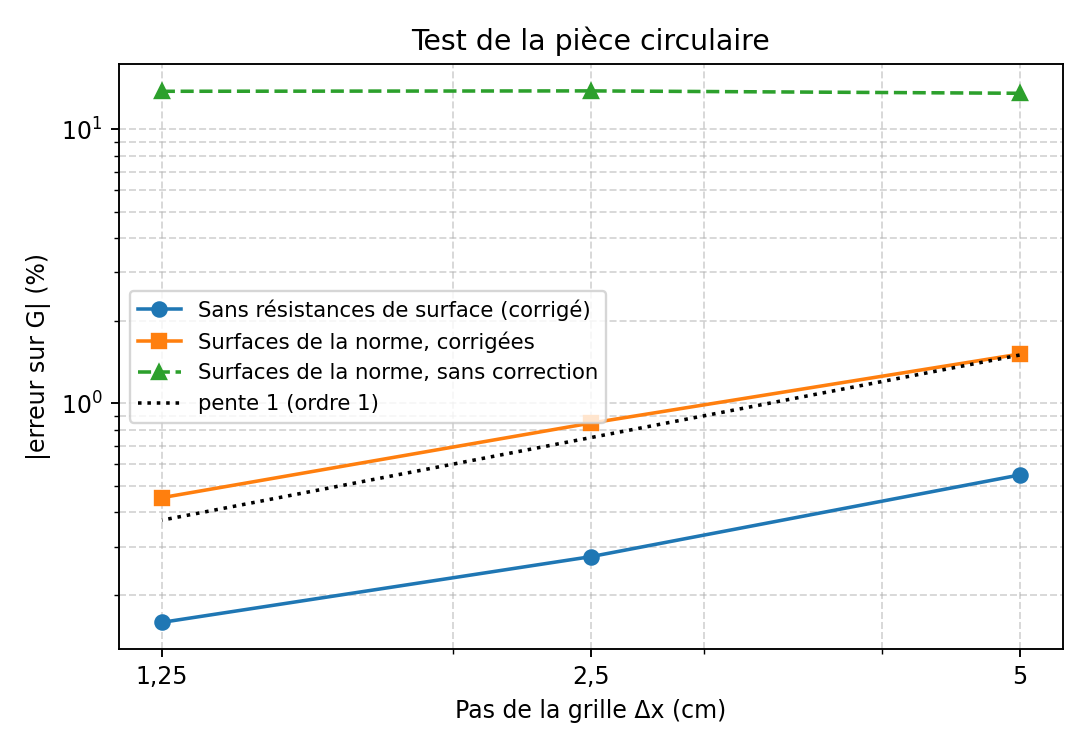
\includegraphics[width=0.62\linewidth]{convergence_test.png}
\caption{Erreur sur $G$ en fonction du pas de la grille (échelles logarithmiques).
Avec les corrections, l'erreur suit une pente 1 ; sans elles, elle reste vers
\qty{14}{\percent}.}
\label{fig-conv}
\end{figure}

Avec les corrections, l'erreur est divisée par 2 quand $\dx$ est divisé par 2 : le
schéma converge à l'ordre 1, et l'erreur reste sous \qty{1}{\percent} dès
\qty{2,5}{\centi\metre}. Sans correction, l'erreur reste d'environ
\qty{14}{\percent} à toutes les résolutions : c'est le facteur d'escalier moyen
0,794 de la \cref{sec-corrections}. Le bilan d'énergie boucle à $10^{-6}$ près dans
tous les cas.

\subsection{Convergence sur les géométries réelles}

Le cercle moyenne les positions des murs par rapport à la grille ; il faut aussi
vérifier les vraies géométries, par raffinement successif ($G$ en
\unit{\watt\per\metre\per\kelvin}, régime établi direct) :

\begin{center}
\begin{tabular}{lccccc}
\toprule
& \qty{5}{\centi\metre} & \qty{3,5}{\centi\metre} & \qty{2,5}{\centi\metre} & \qty{1,25}{\centi\metre} & \qty{0,625}{\centi\metre}\\
\midrule
Carré  & 79,7 & 79,9 & 79,7 & 79,7 & 79,7\\
Koch 0 & 88,4 & 88,5 & 88,6 & 88,8 & 88,8\\
Koch 2 & 117,6 & 117,4 & 118,3 & 118,6 & 119,2\\
Koch 3 & 127,8 & 129,8 & 129,5 & 132,6 & 132,9\\
Koch 4 & 106,3 & 107,2 & 110,7 & 114,4 & 115,5\\
\bottomrule
\end{tabular}
\end{center}

Entre \qty{1,25}{\centi\metre} et \qty{0,625}{\centi\metre} ($2400\times2400$ cases),
$G$ ne varie plus que de \qty{0,03}{\percent} (Koch 0) à \qty{1}{\percent} (Koch 4) :
les valeurs de référence (grille de \qty{1,25}{\centi\metre}) sont justes à environ
\qty{1}{\percent}. Les profondeurs 3 et 4 convergent plus lentement : leurs pointes à
\ang{60} et leurs creux étroits ne sont résolus que par quelques cases sur une grille
grossière. L'ordre des résultats est le même à toutes les résolutions.

\subsection{Défauts trouvés par les tests}\label{sec-defauts}

Chaque test a révélé un défaut que l'observation de la simulation ne montrait pas :
\begin{enumerate}
  \item \textbf{Murs d'un pixel} (version~2) : tracés par l'algorithme de Bresenham,
  ils avaient une résistance trop faible de \qty{15}{\percent} à toutes les
  résolutions (0,843 ; 0,850 ; 0,845). Avec les paramètres d'alors, ce biais était
  masqué par une compensation d'erreurs : un seul cas test ne suffit pas à valider un
  modèle.
  \item \textbf{Précision \texttt{float}} : calcul figé avant le régime établi.
  \item \textbf{Escalier} : surfaces trop conductrices de \qty{20}{\percent} sans
  correction, exactement la valeur théorique.
  \item \textbf{Épaisseur} : invisible sur le cercle (les arrondis s'y compensent),
  révélée en comparant le carré à deux résolutions ($G = 90$ au lieu de 85 dans le
  modèle v3).
  \item \textbf{Grands pas de temps} : champ de l'air faux au-delà de
  \qty{30}{\second} par pas, malgré la stabilité du schéma.
\end{enumerate}

% ===========================================================================
\section{Résultats}\label{sec-resultats}
% ===========================================================================

\subsection{Régime établi}

Régime établi direct sur la grille de \qty{1,25}{\centi\metre} :

\begin{center}
\begin{tabular}{lcccccc}
\toprule
& Périmètre & $\Tair$ moyenne & $\Tair$ max & $G$ & $G/G_{\text{carré}}$ & $G$/périmètre\\
& (m) & (°C) & (°C) & (\unit{\watt\per\metre\per\kelvin}) & & (\unit{\watt\per\square\metre\per\kelvin})\\
\midrule
Carré  & 24,0 & 30,04 & 33,16 & 79,7 & 1,00 & 3,32\\
Koch 0 & 27,4 & 29,01 & 32,24 & 88,8 & 1,11 & 3,25\\
Koch 1 & 31,6 & 28,00 & 31,15 & 100,0 & 1,26 & 3,17\\
Koch 2 & 40,0 & 26,75 & 29,91 & 118,6 & 1,49 & 2,97\\
Koch 3 & 52,1 & 26,03 & 29,20 & \textbf{132,6} & \textbf{1,66} & 2,54\\
Koch 4 & 68,9 & 26,99 & 30,17 & 114,4 & 1,44 & 1,66\\
\bottomrule
\end{tabular}
\end{center}

\begin{figure}[H]
\centering
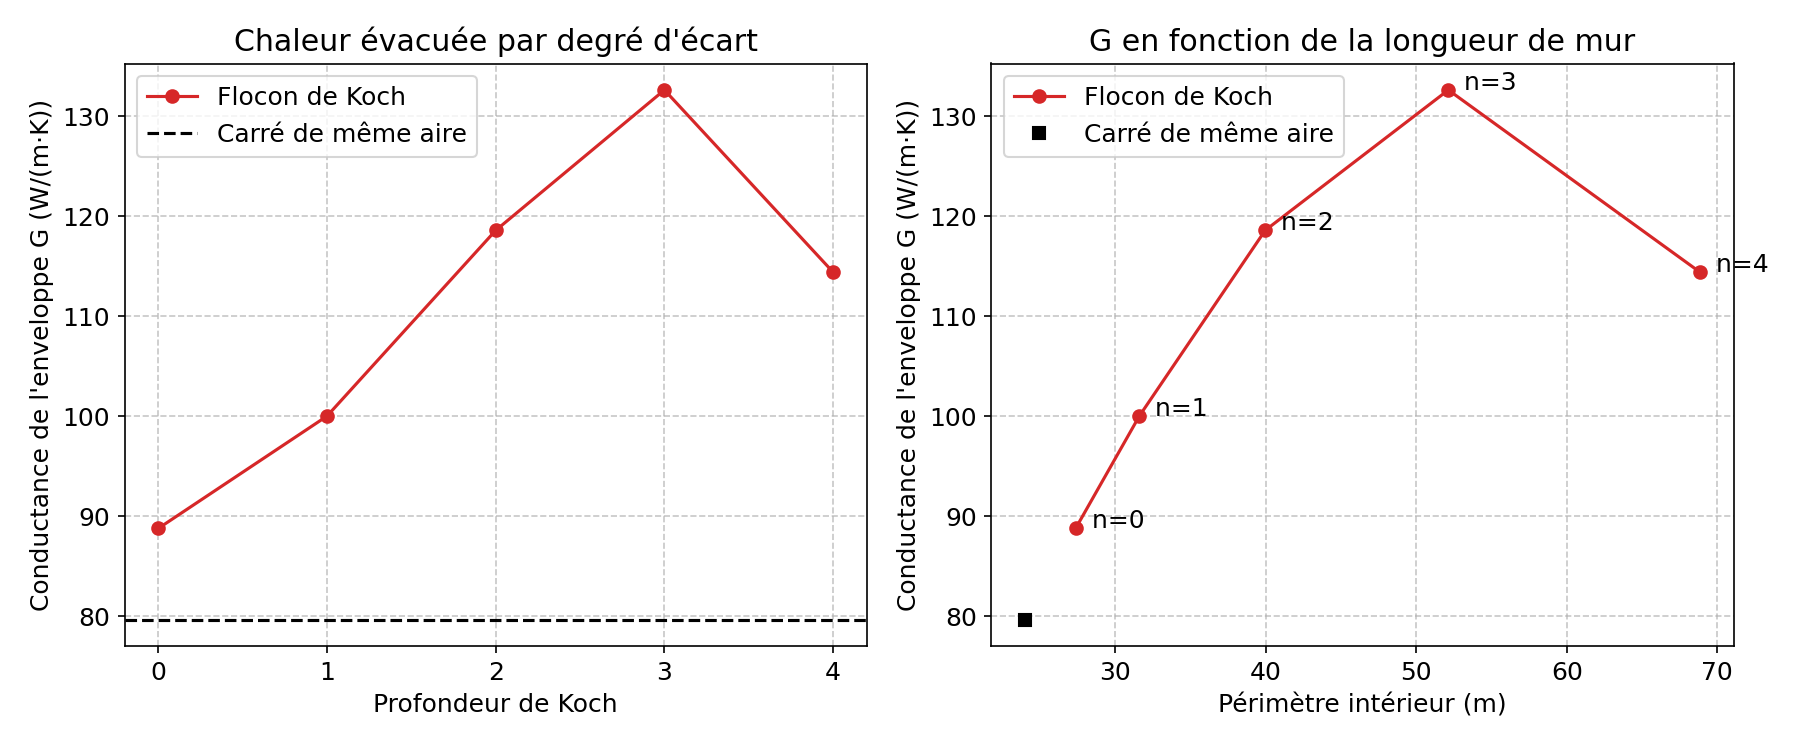
\includegraphics[width=\linewidth]{profondeur.png}
\caption{Conductance de l'enveloppe en fonction de la profondeur (à gauche) et du
périmètre intérieur (à droite). La ligne pointillée est le carré.}
\label{fig-profondeur}
\end{figure}

\subsection{Interprétation}

\begin{itemize}
  \item \textbf{La fractale évacue mieux.} Avec la même source, le flocon de profondeur
  3 reste à \qty{26,0}{\degreeCelsius} contre \qty{30,0}{\degreeCelsius} pour le
  carré : il évacue \qty{66}{\percent} de chaleur en plus par degré d'écart.
  \item \textbf{Les rendements sont décroissants.} Le périmètre augmente de
  \qty{117}{\percent} entre le carré et la profondeur 3, mais $G$ seulement de
  \qty{66}{\percent} : chaque mètre de mur sert de moins en moins (dernière colonne,
  à comparer à $U = 3,52$). Trois raisons : dans les creux, les murs voisins se
  partagent la même chaleur ; la surface extérieure du mur est plus courte que la
  surface intérieure ; et la chaleur doit traverser l'air jusqu'aux pointes,
  éloignées de la source.
  \item \textbf{Il existe une profondeur optimale, ici 3.} À la profondeur 4, les
  détails (\qty{9}{\centi\metre}) sont plus petits que le mur (\qty{20}{\centi\metre}).
  Le mur, dilatation du contour, bouche les creux : sa surface extérieure raccourcit
  (sur la grille fine, les faces mur/extérieur passent de 5\,100 à 3\,916), tandis que
  le béton s'épaissit localement. $G$ chute alors de \qty{14}{\percent}. C'est la
  limite physique prévue en \cref{sec-nmax}.
  \item \textbf{Le rôle de l'air.} Dans le modèle v3, où l'air avait une seule
  température, le gain de la profondeur 3 était de \qty{76}{\percent}. La résistance
  de l'air entre la source et les murs pénalise les parties éloignées de la source,
  donc les pointes : le gain réel dépend du brassage de l'air.
\end{itemize}

\subsection{Évolution dans le temps}

\begin{figure}[H]
\centering
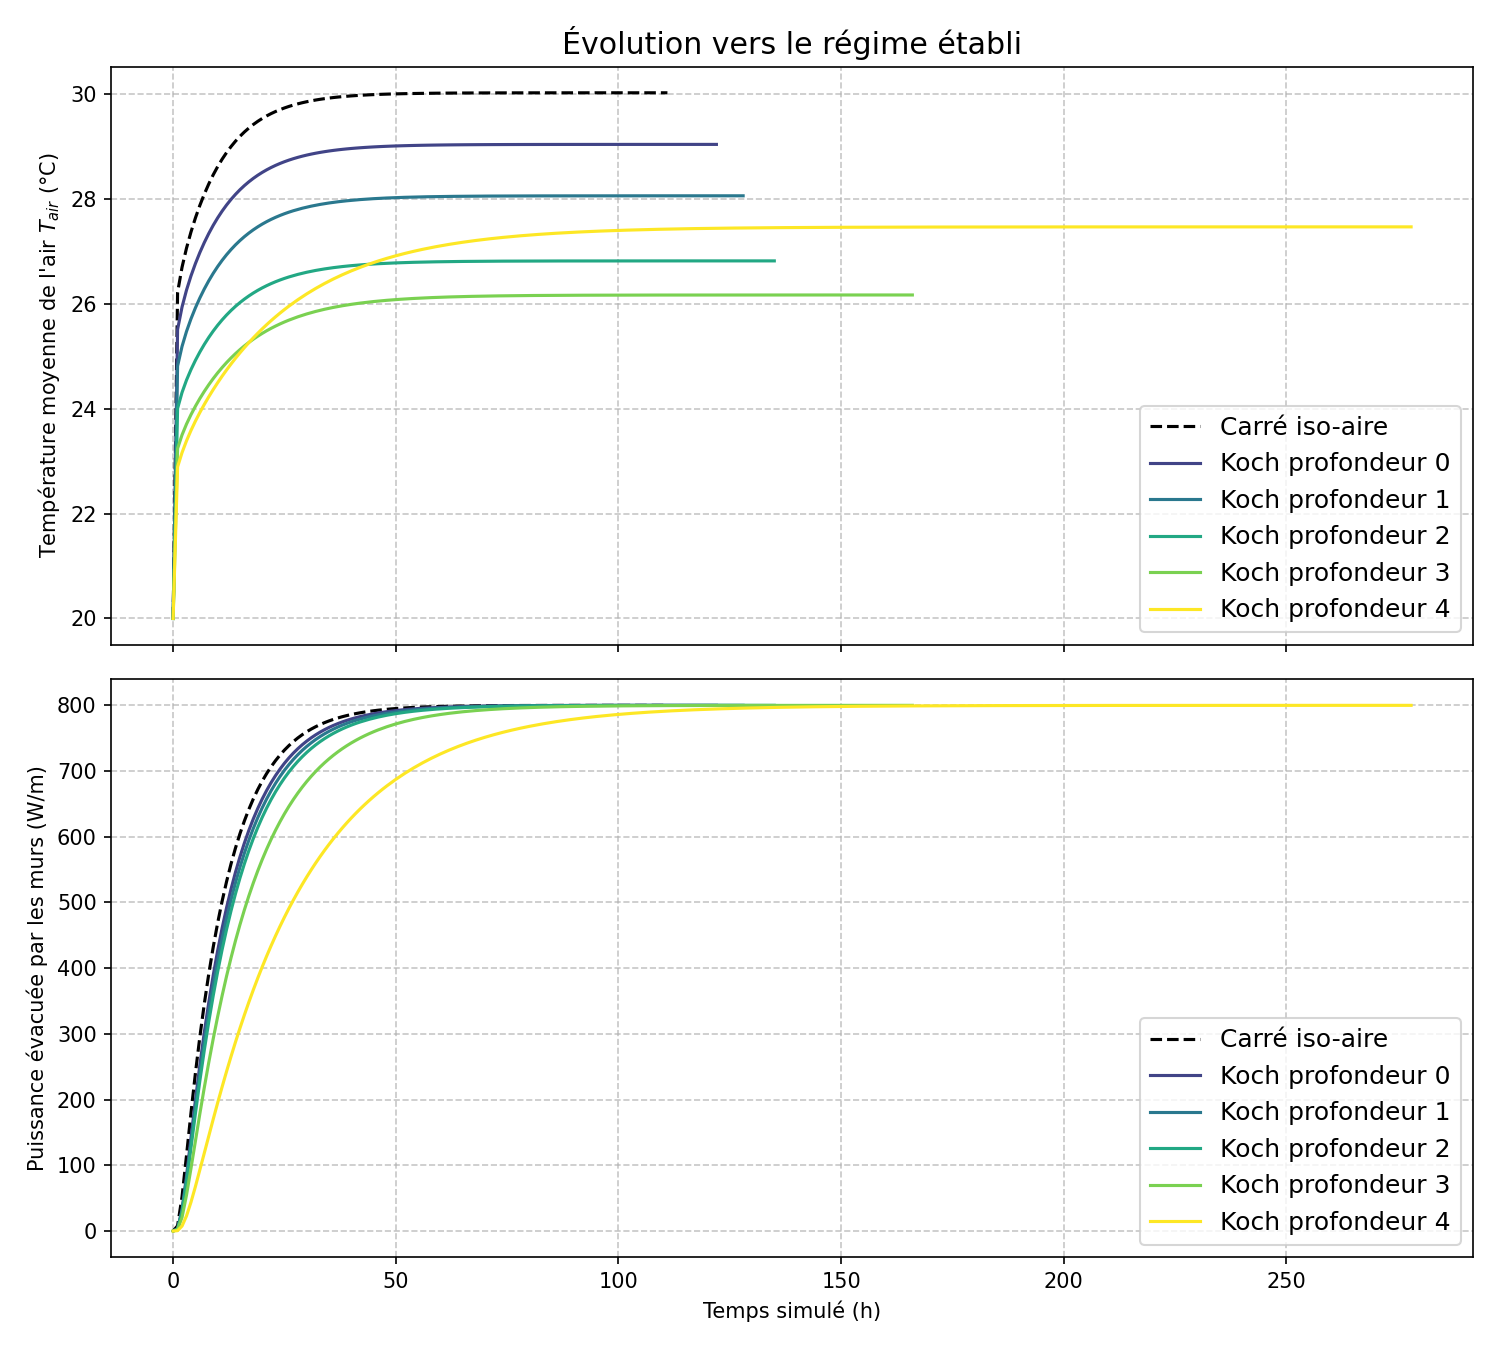
\includegraphics[width=0.82\linewidth]{temps.png}
\caption{Température moyenne de l'air et puissance évacuée par les murs, de la mise
en route au régime établi (grille de la fenêtre).}
\label{fig-temps}
\end{figure}

La température de l'air monte en quelques minutes (l'air a peu de capacité), puis
suit lentement l'échauffement des murs. La puissance évacuée croît jusqu'à
\qty{800}{\watt\per\metre} : c'est le bilan d'énergie en régime établi. Le régime établi
(à $10^{-5}$ près) est atteint après \qty{111}{\hour} pour le carré, de 122 à
\qty{166}{\hour} pour les profondeurs 0 à 3, et \qty{278}{\hour} pour la profondeur 4,
qui a le plus de béton à chauffer et dont les murs évacuent le moins bien.

\subsection{Ce que montre la fenêtre}

\begin{figure}[H]
\centering
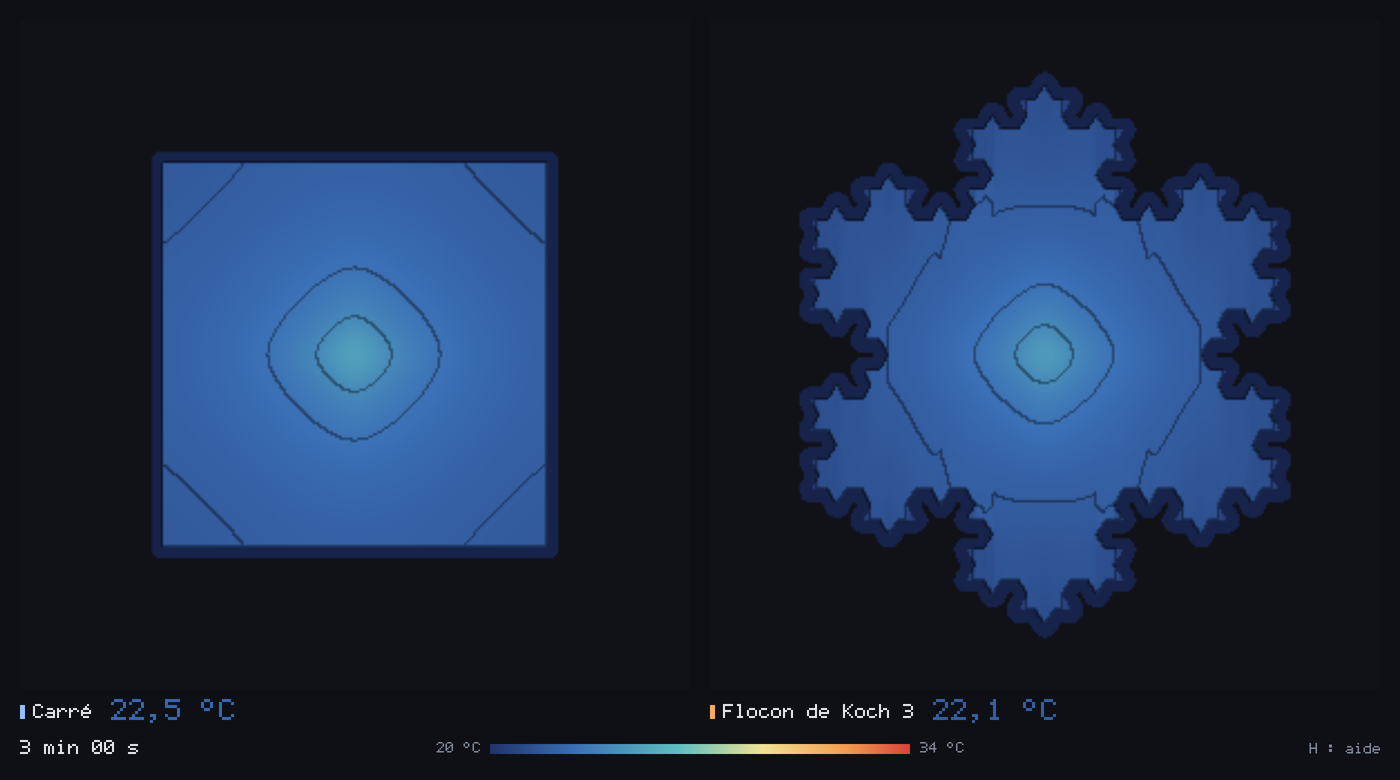
\includegraphics[width=\linewidth]{debut.png}
\caption{Après 3 minutes : la chaleur quitte la source. Les isothermes sont presque
circulaires ; les pointes du flocon, loin de la source, sont encore froides.}
\end{figure}

\begin{figure}[H]
\centering
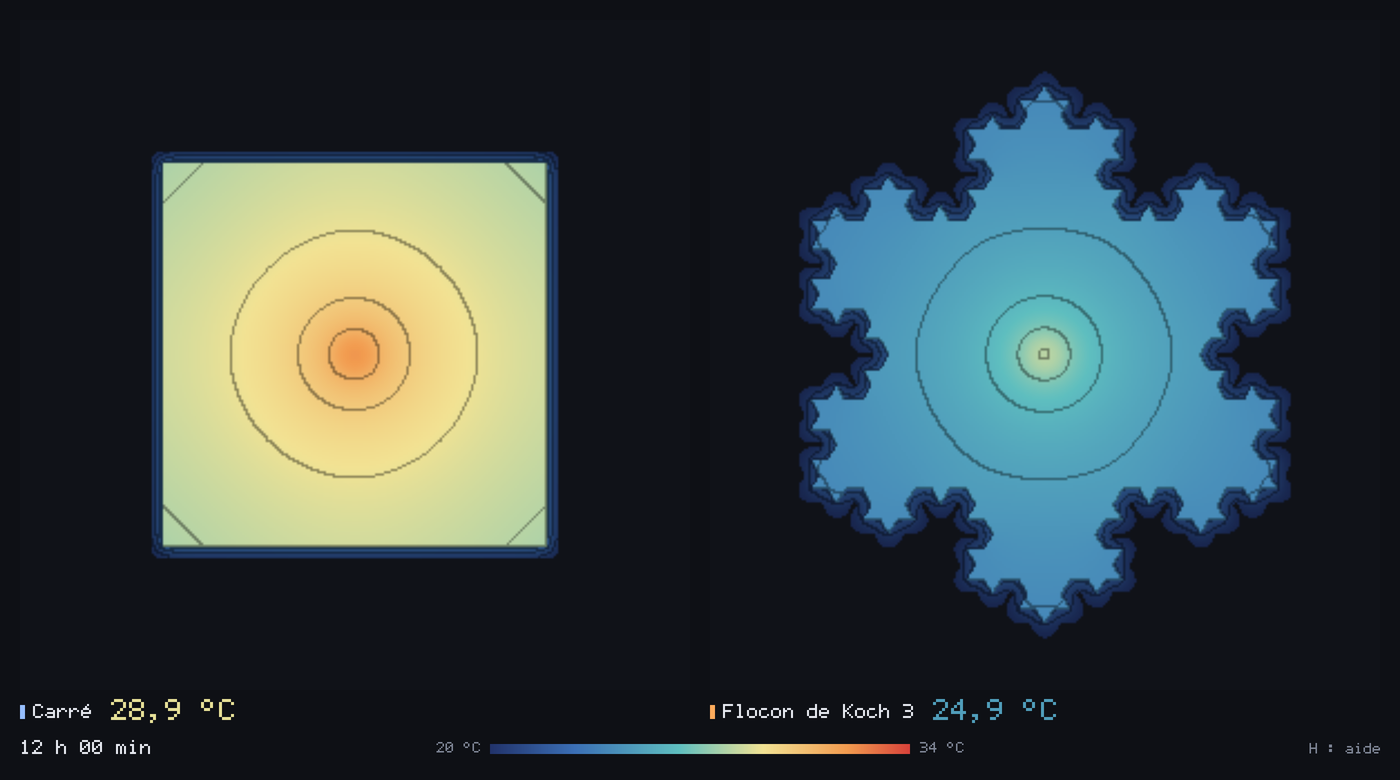
\includegraphics[width=\linewidth]{12h.png}
\caption{Après 12 heures : les murs chauffent ; avec la même source, le flocon reste
plus frais que le carré.}
\end{figure}

\begin{figure}[H]
\centering
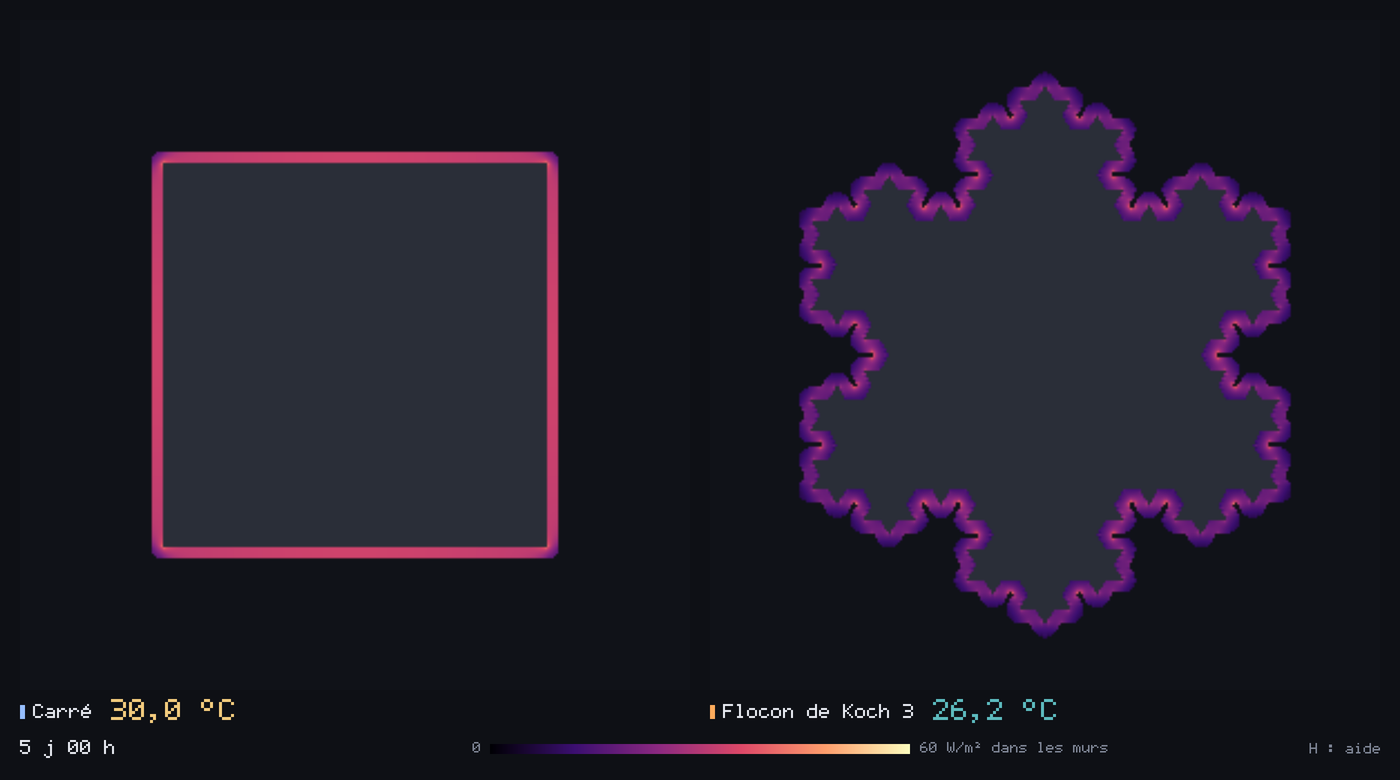
\includegraphics[width=\linewidth]{flux.png}
\caption{Vue flux en régime établi : le mur du carré évacue uniformément ; dans le
flocon, les pointes évacuent beaucoup et le fond des creux très peu.}
\end{figure}

% ===========================================================================
\section{Limites et perspectives}\label{sec-limites}
% ===========================================================================

\begin{enumerate}
  \item \textbf{Conductivité effective de l'air.} La convection est représentée par
  une diffusion. $\la$ fixe la répartition de la chaleur dans la pièce et pèse sur le
  gain de la fractale ; une étude de sensibilité est nécessaire.
  \item \textbf{Position de la source.} Une source près d'un mur, ou plusieurs sources
  (occupants), modifieraient la comparaison.
  \item \textbf{Extérieur à température fixe.} En canicule, l'extérieur est plus chaud
  que l'intérieur, et la fractale ferait entrer plus de chaleur. Un cycle jour/nuit,
  où le bilan dépend de l'inertie des murs, est l'étape naturelle pour la question
  climatique.
  \item \textbf{Mur non isolé.} Avec un isolant, la résistance du mur domine et le rôle
  de la forme change.
  \item \textbf{Contrôle.} Comparer la fractale à une forme non fractale de même
  périmètre (carré crénelé) dirait si c'est la fractale qui compte, ou seulement la
  longueur du mur.
  \item \textbf{Passage en trois dimensions.} Une vraie pièce, avec sol et plafond, où
  l'air chaud monte, ou une fractale en volume (surface de Koch, éponge de Menger).
  Les méthodes se transposent : les directions alternées deviennent trois passes de
  systèmes tridiagonaux, et le gradient conjugué reste valable, pour $N = N_g^3$
  inconnues.
\end{enumerate}

% ===========================================================================
\section{Conclusion}
% ===========================================================================

À aire égale et pour une même source, une pièce en flocon de Koch évacue nettement
mieux la chaleur qu'une pièce carrée : \qty{66}{\percent} de plus par degré d'écart à
la profondeur 3, soit \qty{4}{\degreeCelsius} de moins dans la pièce. Le gain n'est
pas proportionnel à l'allongement du mur, et il s'inverse à la profondeur 4 : quand les
détails deviennent plus fins que l'épaisseur du mur, celui-ci les bouche. Une fractale
« réelle » est toujours tronquée, et son intérêt thermique a un optimum fixé par la
matière qui la constitue.

Sur le plan méthodologique, le projet montre l'intérêt de valider un modèle avant de
l'exploiter : chaque test confronté à une solution exacte ou à un raffinement de
maillage a révélé un défaut que la simulation, visuellement convaincante, ne laissait
pas soupçonner. Le modèle actuel est conservatif, validé à moins de \qty{1}{\percent},
et ses résultats sont indépendants de la grille à environ \qty{1}{\percent} près. Il
constitue une base solide pour les étapes suivantes : sensibilité au brassage de
l'air, cycle jour/nuit et passage en trois dimensions.

\appendix

% ===========================================================================
\section{Paramètres du modèle}
% ===========================================================================

\begin{center}
\begin{tabular}{llr}
\toprule
Grandeur & Symbole & Valeur\\
\midrule
Aire intérieure & $A$ & \qty{36}{\square\metre}\\
Épaisseur du mur & $e$ & \qty{0,20}{\metre}\\
Conductivité du béton & $\lm$ & \qty{1,75}{\watt\per\metre\per\kelvin}\\
Capacité volumique du béton & $\rho c$ & \qty{2,3e6}{\joule\per\cubic\metre\per\kelvin}\\
Conductivité effective de l'air & $\la$ & \qty{100}{\watt\per\metre\per\kelvin}\\
Capacité volumique de l'air & $\rho c$ & \qty{1206}{\joule\per\cubic\metre\per\kelvin}\\
Résistance superficielle intérieure & $\Rsi$ & \qty{0,13}{\square\metre\kelvin\per\watt}\\
Résistance superficielle extérieure & $\Rse$ & \qty{0,04}{\square\metre\kelvin\per\watt}\\
Puissance de la source & $Q$ & \qty{800}{\watt\per\metre}\\
Rayon de la source & $r_s$ & \qty{0,30}{\metre}\\
Température extérieure et initiale & $\Text$ & \qty{20}{\degreeCelsius}\\
Pas de temps maximal & $\dt$ & \qty{30}{\second}\\
Grille de la fenêtre & & $300\times300$, $\dx = \qty{3,5}{\centi\metre}$\\
Grille des résultats & & $1200\times1200$, $\dx = \qty{1,25}{\centi\metre}$\\
\bottomrule
\end{tabular}
\end{center}

% ===========================================================================
\section{Reproduire les résultats}
% ===========================================================================

\begin{lstlisting}[language=bash,numbers=none,caption={Commandes, depuis la racine du dépôt}]
brew install sdl2 pkg-config      # macOS
make                              # compile ./thermalfractalsim
make run                          # fenetre interactive
make test                         # validation (solution exacte, 3 resolutions)
make data                         # courbes dans le temps (res_*.csv)
make regime                       # regime etabli sur grille fine (regime_*.csv)
make plot                         # graphiques
python3 docs/rapport/figures/generer_figures.py   # figures du rapport
make rapport                      # ce document
\end{lstlisting}

\end{document}
